\documentclass{article}
\title{\textbf{Notes on Geometric Learning}}
\author{Matthew Mo}
\date{\today}

\usepackage{ctex, xeCJK, zxjatype}
\usepackage{metalogo, makecell, svg, amssymb, amsfonts, amsmath, physics, fancyhdr, geometry, graphicx, pdfpages, ragged2e, bm}
\usepackage{verbatim}
\newcommand{\R}{\mathbb{R}}
\newcommand{\rarr}{\rightarrow}
\newcommand{\lop}{Laplace算子}
\newcommand{\tRarr}{$\Rightarrow$}
\newcommand{\trarr}{$\Rightarrow$}
\newcommand{\filter}{\Gamma_{l,l'}}
\newcommand{\fn}[1]{\footnote{#1}}
\newcommand{\bs}[1]{\boldsymbol{#1}}
\newcommand{\iprod}[2]{\langle #1, #2 \rangle}
\newcommand{\define}{\textbf{Definition} }
\newcommand{\trm}{\textbf{Theorem} }
\newcommand{\alg}{\textbf{Algorithm} }
\newcommand{\cov}{\text{Cov}}
\newcommand{\bb}{\mathbb}
\newtheorem{theorem}{Theorem}[section]
\newtheorem{lemma}[theorem]{Lemma}
\newtheorem{proposition}[theorem]{Proposition}
\newtheorem{corollary}[theorem]{Corollary}
\newtheorem{definition}[theorem]{Definition}

\newenvironment{proof}[1][Proof]{\begin{trivlist}
\item[\hskip \labelsep {\bfseries #1}]}{\end{trivlist}}
% \newenvironment{definition}[1][Definition]{\begin{trivlist}
% \item[\hskip \labelsep {\bfseries #1}]}{\end{trivlist}}
\newenvironment{example}[1][Example]{\begin{trivlist}
\item[\hskip \labelsep {\bfseries #1}]}{\end{trivlist}}
\newenvironment{idea}[1][Idea]{\begin{trivlist}
\item[\hskip \labelsep {\bfseries #1}]}{\end{trivlist}}
\newenvironment{remark}[1][Remark]{\begin{trivlist}
\item[\hskip \labelsep {\bfseries #1}]}{\end{trivlist}}
\renewcommand{\cal}{\mathcal}
\usepackage[hidelinks, bookmarks]{hyperref} % add index hyper-links
\newcommand{\coro}{\textbf{Corollary} }
\newcommand{\tgt}{\textbf{Target} }
\newcommand{\bt}[1]{\textbf{#1}}
\newcommand{\lp}{Lagrange Polynomial}
\newcommand{\np}{Newton Polynomial}
\newcommand{\where}{\text{where }}
\newcommand{\centerimage}[2]{
    \centerline{\includegraphics[width=#1\paperwidth]{#2}
    }
}
\let\titleoriginal\title           % save original \title macro
\newcommand{\thetitle}{}
\renewcommand{\title}[1]{          % substitute for a new \title
    \titleoriginal{#1}%               % define the real title
    \renewcommand{\thetitle}{#1}        % define \thetitle
}

\newCJKfontfamily\gothic{IPAexGothic}
\newCJKfontfamily\mincho{IPAexMincho}

% set plain style
\pagestyle{fancy}
\lhead{} 
\chead{} 
\rhead{} 
% \lfoot{\it Notes on Geometric Learning} 
\lfoot{\hyperref[contents]{\thetitle}} 
% \lfoot{\thetitle} 
\cfoot{}
\rfoot{\thepage} 


% Length to control the \fancyheadoffset and the calculation of \headline
% simultaneously
\newlength\FHoffset
\setlength\FHoffset{1cm}

\addtolength\headwidth{2\FHoffset}

\fancyheadoffset{\FHoffset}

% these lengths will control the headrule trimming to the left and right 
\newlength\FHleft
\newlength\FHright

% here the trimmings are controlled by the user
\setlength\FHleft{1cm}
\setlength\FHright{0cm}

% The new definition of headrule that will take into acount the trimming(s)
\newbox\FHline
\setbox\FHline=\hbox{\hsize=\paperwidth%
  \hspace*{\FHleft}%
  \rule{\dimexpr\headwidth-\FHleft-\FHright\relax}{\headrulewidth}\hspace*{\FHright}%
}
\renewcommand\headrule{\vskip-.7\baselineskip\copy\FHline}

\renewcommand{\headrulewidth}{0.7pt} % hline width
\renewcommand{\footrulewidth}{0.7pt} 

% set margin
\geometry{a4paper,scale=0.75}
\newcommand{\note}{\textbf{Note} }
\begin{document}
\maketitle
\tableofcontents
\section{NeVAE}
    \bt{Idea} VAE on graph, node-wise repr, permutation invariant.
    
    \centerline{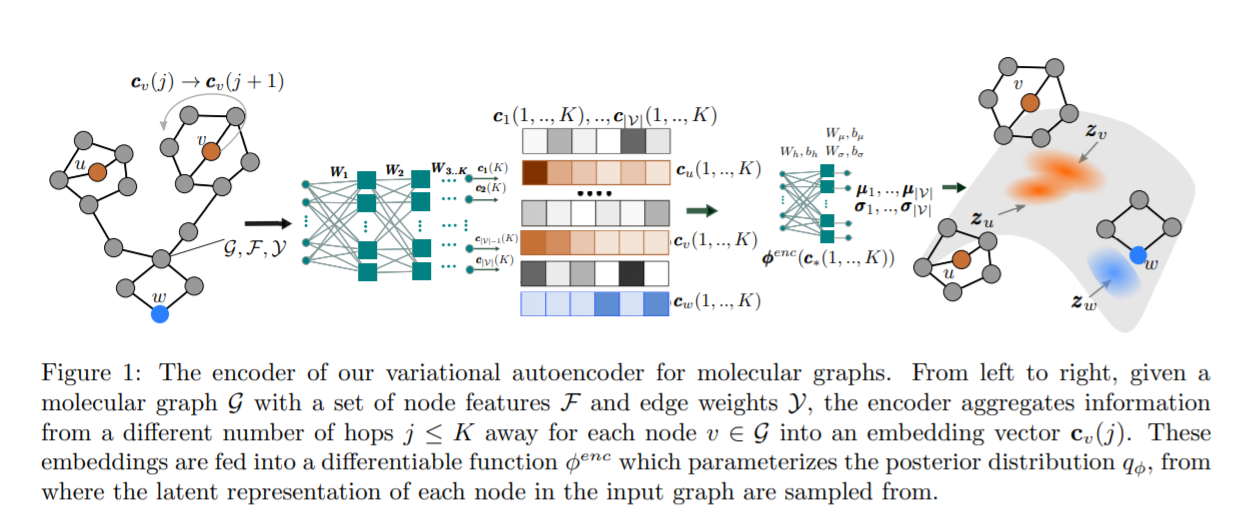
\includegraphics[width=0.85\paperwidth]{nevae-enc.PNG}}

    Encoder: GNN-like message-passing on k-hops:
    \begin{align}
        &q_\phi(\bs z_u|\mathcal{V,E,F,Y})\sim\mathcal{N}(\bs \mu_u,Diag(\bs \sigma_u))\\
        &[\bs \mu_u, \bs \sigma_u]=\phi^{enc}({\bs c_u(k)}_{k=1..K})\\
        &\bs c_u(k)=
        \begin{cases}
            &\bs r(\bs W_k^\mathcal{T}\bs t_u + \bs W_k^\mathcal{X}\bs x_u),k=1\\
            &\bs r(\bs W_k^\mathcal{T}\bs t_u + \bs W_k^\mathcal{X}\bs x_u\odot \bs \Lambda(\{y_{uv} \bs c_v(k-1)\}_v\in N(u))),k>1
        \end{cases}
    \end{align}

    \centerline{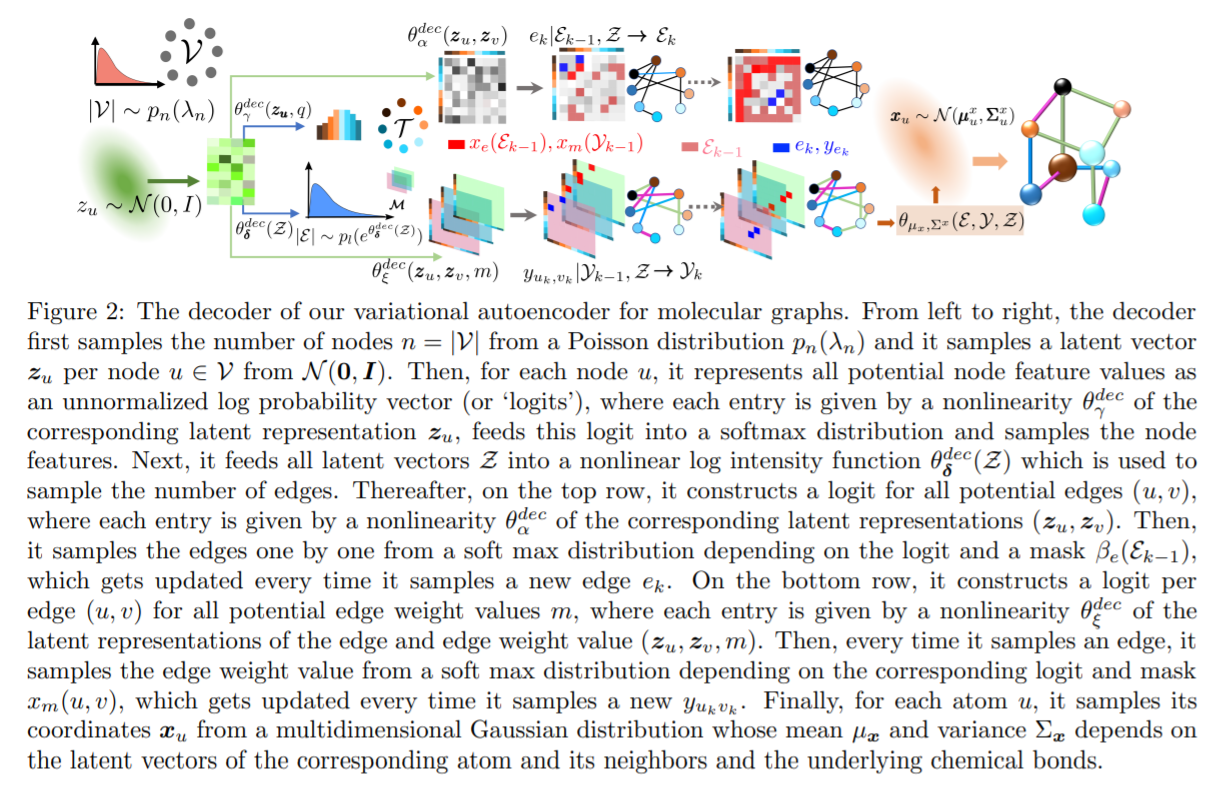
\includegraphics[width=0.85\paperwidth]{nevae-arch.PNG}}

    Decoder: genetate logits, softmax edges one-by-one, possible binary mask(for expert exp.).
    \begin{align}
        &\text{Nodes Count:} |\mathcal{V}|\sim p_l(\lambda_n)\\
        &\text{Latent Repr.:} {\bs z_u}\sim \mathcal{N}(\bs 0,\bs I)\\
        &\text{Node Feat.:} \bs f_u=softmax_u(\theta_{\bs \gamma}^{dec}(\bs z_u, q)),q \text{is atom type}\\
        &\text{Edges Count:} |\mathcal{E}|\sim p_l(e^{\theta_{\bs \delta}^{dec}(\mathcal{Z})})\\
        &\text{Edges Gen.:} p(e=(u,v)|\mathcal{E}_{k-1},\mathcal{V})=\frac{\beta_e e^{\theta^{dec}_{\bs \alpha}(\bs z_u, \bs z_v)}}{\sum_{e'=(u',v')\not \in \mathcal{E}_{k-1}} \beta_{e'} e^{\theta^{dec}_{\bs \alpha}(\bs z_u', \bs z_v')}}\\
        &\text{E. Feat. Gen.:} p(y_{uv}=m|\mathcal{Y}_{k-1},\mathcal{V})=\frac{\beta_m(u,v) e^{\theta^{dec}_{\bs \xi}(\bs z_u, \bs z_v, m)}}{\sum_{m'\not=m \beta_m'(u,v) e^{\theta^{dec}_{\bs \xi}(\bs z_u, \bs z_v, m')}}},\text{note: not normal softmax?}\\
        &\text{Pos. Gen.:} p(\bs x_u|\mathcal{E,Y,Z})=\mathcal N(\bs \mu_x, \bs \Sigma_x)\\
        &[\bs \mu_x, \bs \Sigma_x]=[]
    \end{align}
    %...

\section{Seminar on Self/Un-Supervised Learning @ 2020/9/16}
\subsection{Self-Learning @ Video Learning}
    Supervised success: good \& sufficient data, a way different from human! \tRarr \textit{Linda Smith, The Dev. of Embodied Cognition}

    \bt{Paragidims}:
    \begin{itemize}
        \item Use proxy task(e.g. semantics repr.) for a repr., use linear probing for downstream task.
        \item Use proxy task(e.g. semantics repr.) for a repr., generalizable with \textit{zero annotation}
    \end{itemize}
    
    \bt{Why video-based self-supervised}: like what human percepts, rich info; might with audio.

    Proxy loss design: temporal info, spatial cohenrence, motions of obj., multimodal
    
    \bt{Temporal}:
    \begin{itemize}
        \item shuffle \& learn
        \item forward or backward?(arrow of time)
        \item SpeedNet: which speed(frame-rate) is normal/speed-up 
        \item ===Weak, irrelative with downstream tasks===
        \item DPC: \textit{learn repr. in predicting future in video}
    \end{itemize}

    \centerline{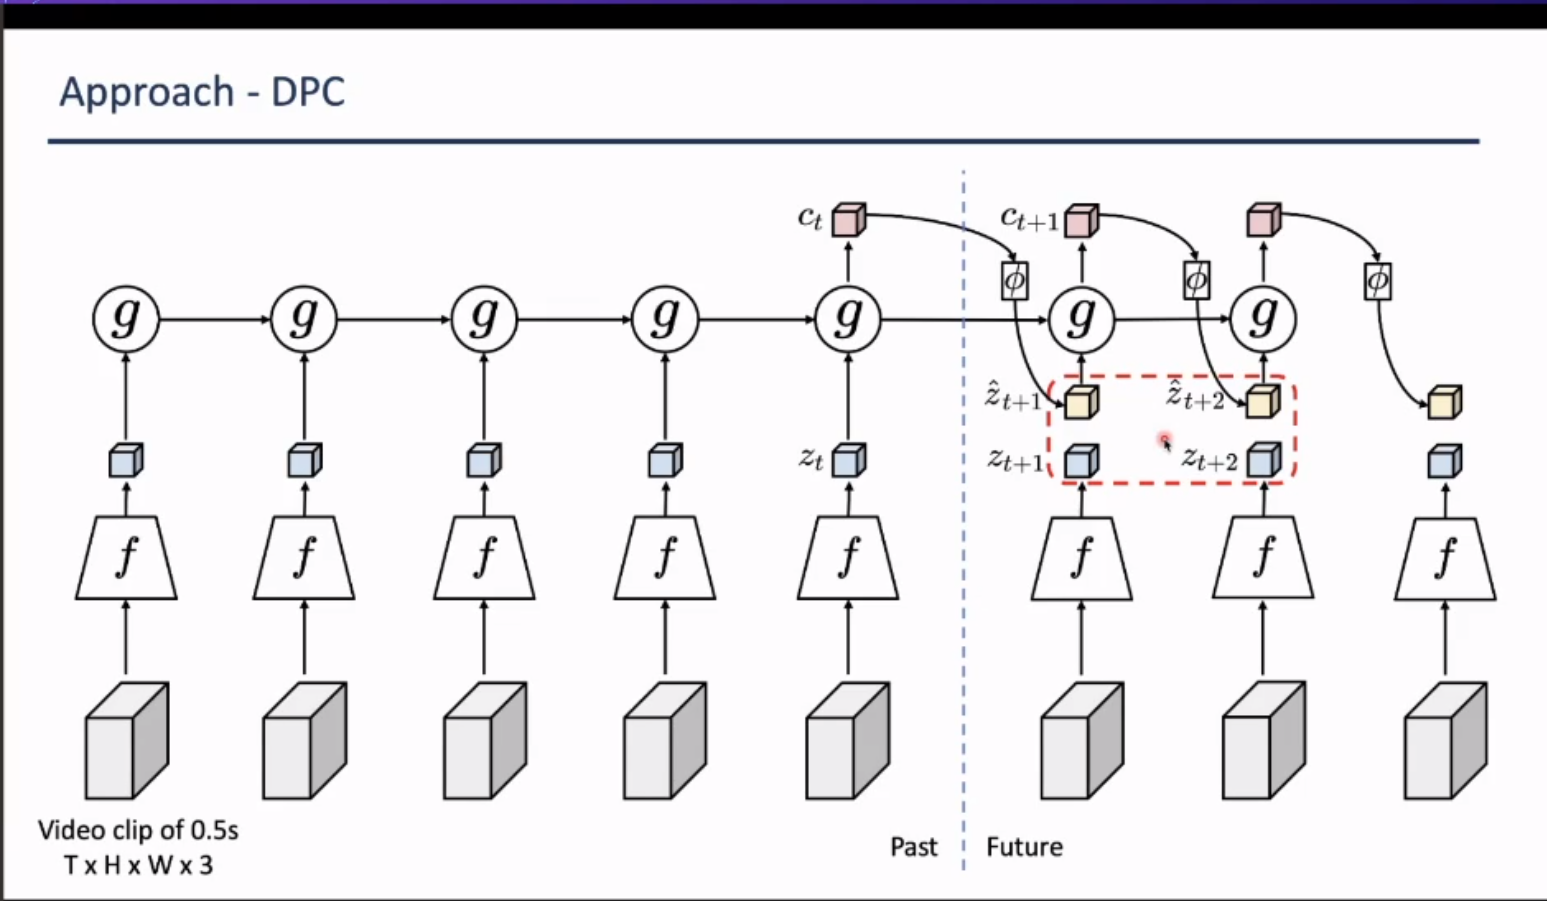
\includegraphics[width=0.8\paperwidth]{dpc-arch.PNG}}
    DPC Arch.:encoder-decoder like, contrast learning(infoNCE)

    \centerline{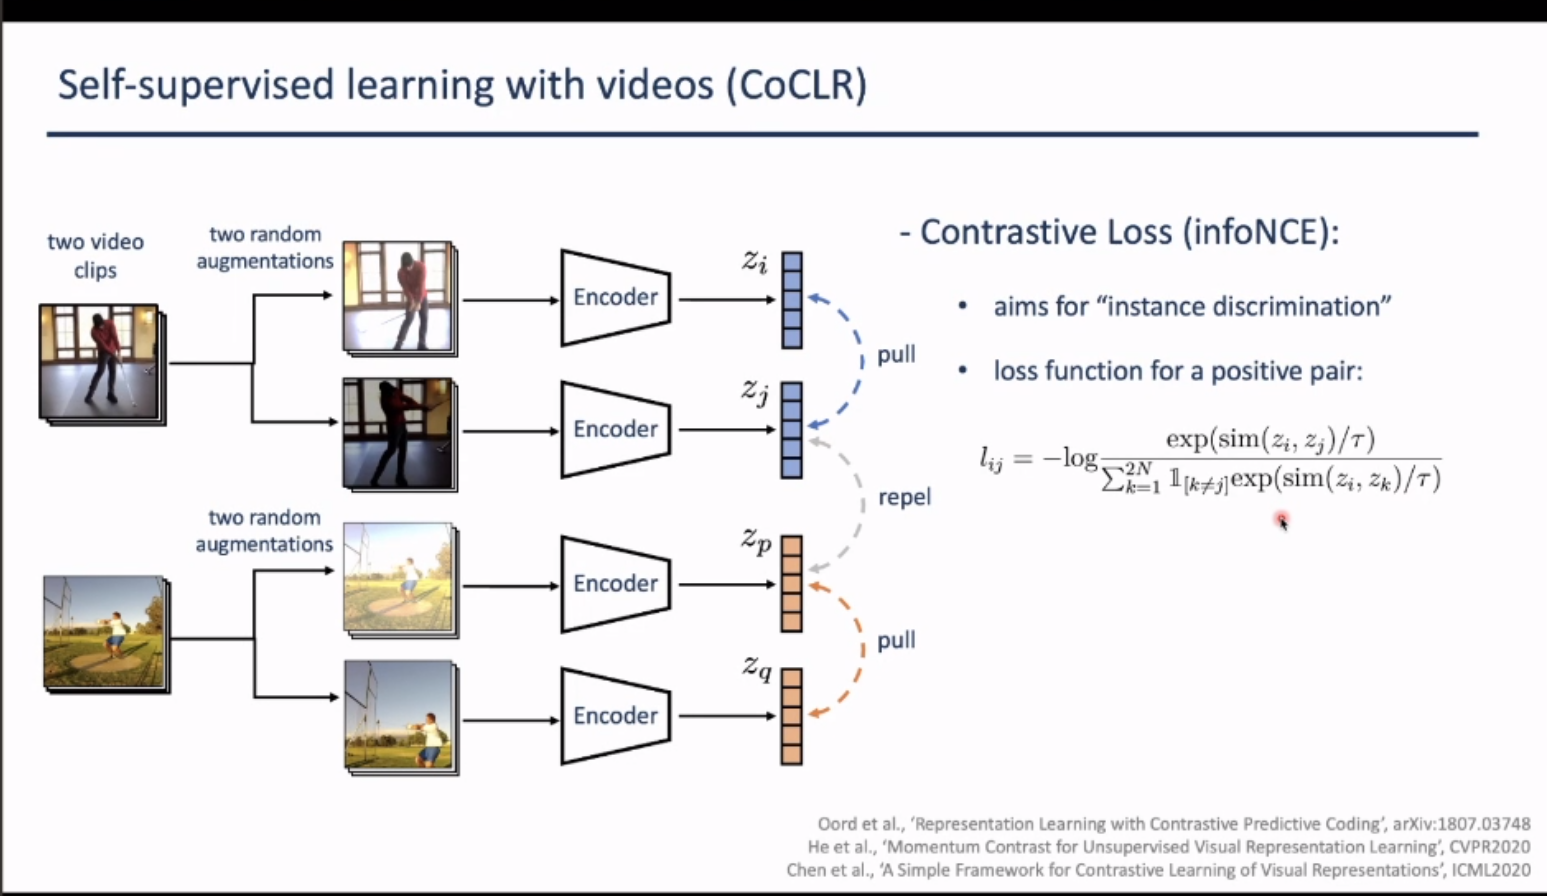
\includegraphics[width=0.8\paperwidth]{coclr.PNG}}
    \centerline{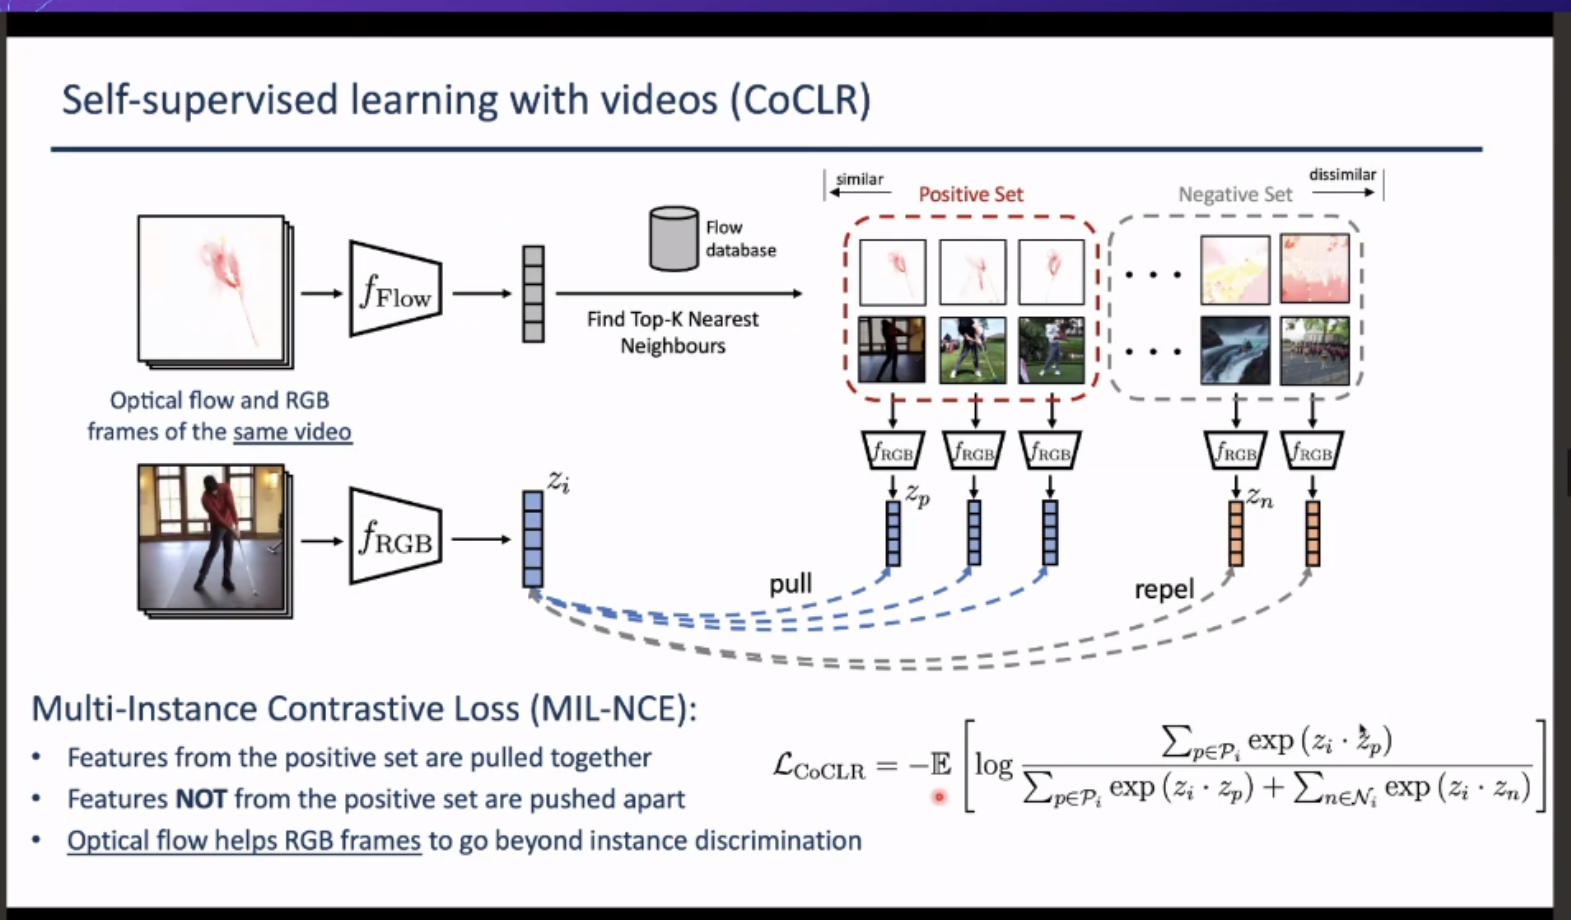
\includegraphics[width=0.8\paperwidth]{coclr2.PNG}}
    CoCLR: SimCLR like(infoNCE), colearning multimodally with motion flow(MIL-NCE, with noise added)

    Audio-Video Co-learning: train a net to check if image/audio clip are same-sourced! Get both video/audio repr.

    MAST: self-supervised tracking, give 1st frame mask(seg.), predict sequantial segmentations

    \bt{Next}:
    \begin{itemize}
        \item More efficient learning
        \item Scale up model to uncurrated data, like GPT-1/2/3
        \item Design proxy task for obj-centric learing
        \item Design and understand \bt{effective memory!!!}(for video task especially)
        \item Hand-crafted proxy task \trarr Auto proxy task design?
        \item Theoratic: small or negative improvement, in upstream task to downstream task.
        \item Are there difficult task for supervised learning but easy for SSL(e.g. unable to label)?
    \end{itemize}

\subsection{Transformation Equivariance vs. Invariance @ Visial Repr. Learning}
    \bt{Contents}:
    \begin{itemize}
        \item TER(Transformation Equivariance Repr.)
        \item AET(AutoEncoding Transformation)
        \item AVT(Autoencoding Variational Transformation)
        \item SAT(Semi-supervised Autoencoding Transformation)
    \end{itemize}

    CNN = Translation Equivariant Repr. + FC Classifier. Go beyond: Tranformation Equivariant Repr. + Tranformation Invariant Classifier

    Trans. Equiv.: $E(\bs t(\bs x))=\bs \rho(\bs t)[E(\bs x)]$. Trans. Inv. is when $\bs \rho \equiv \bs 1_E$.

    Steerability: $\bs \rho$ is inpend. with sample $\bs x$.

    Targets: Non-linear $\bs \rho$, General Transformation(e.g. recoloring)

    \centerline{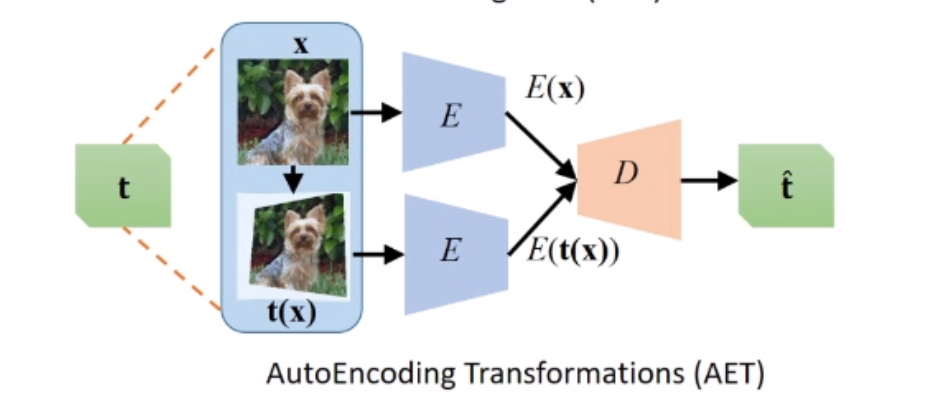
\includegraphics[width=0.8\paperwidth]{aet.PNG}}
    \centerline{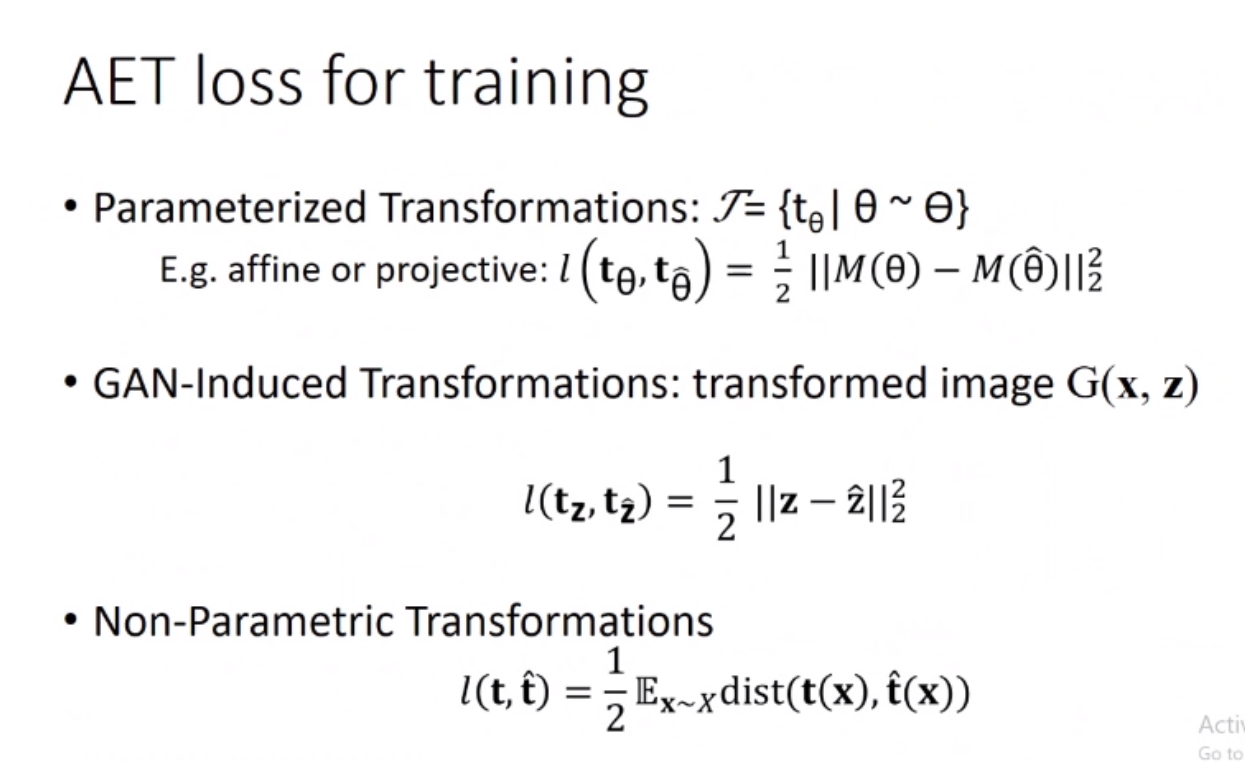
\includegraphics[width=0.8\paperwidth]{aetloss.PNG}}
    AET:\begin{itemize}
        \item use autoencoders to learn \bt{transformations}
        \item trans. generated randomly for self-supervised learing
        \item use Siamese net as encoder backbone
        \item AET loss: parameterized, non-parametric, GAN-induced
    \end{itemize}
    
    \centerline{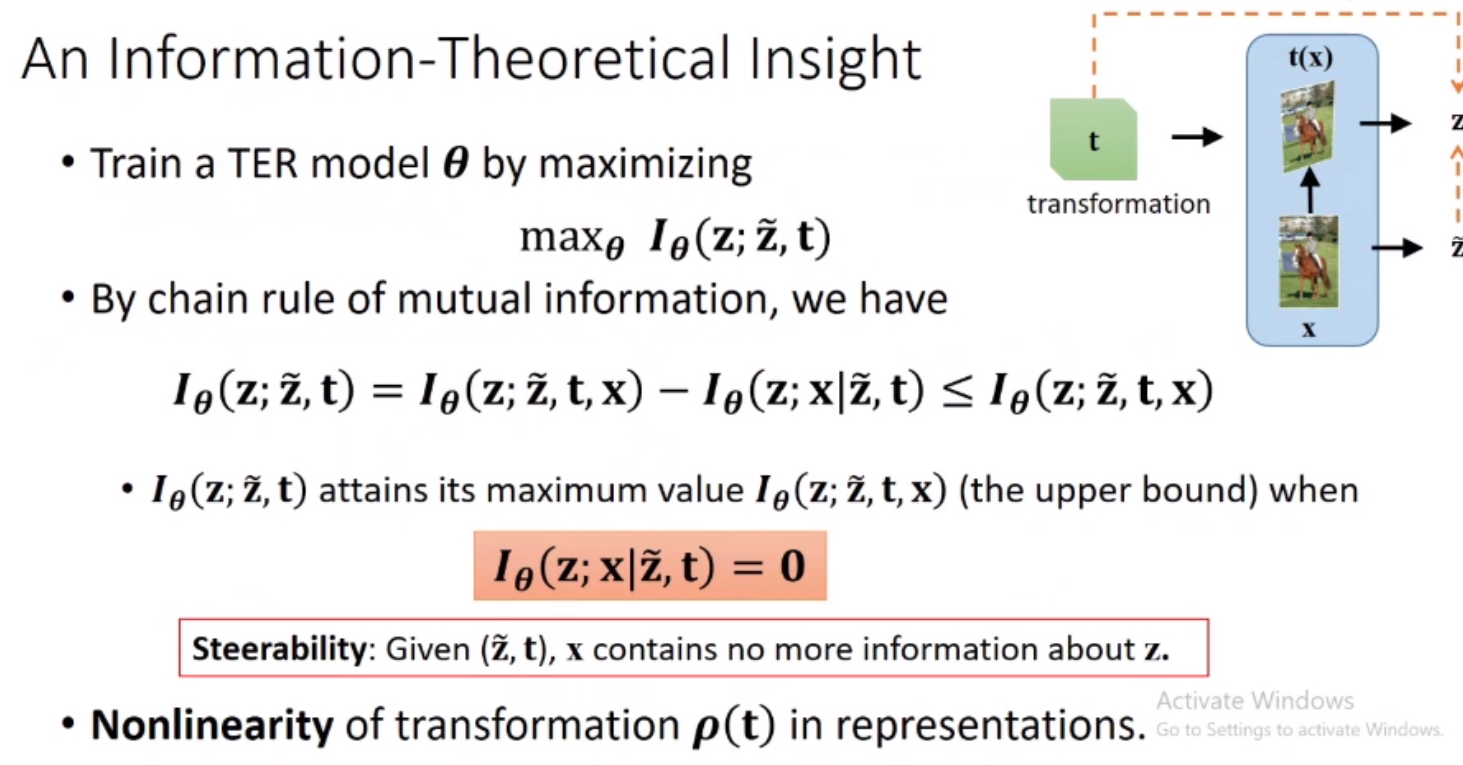
\includegraphics[width=0.8\paperwidth]{avt.PNG}}
    \centerline{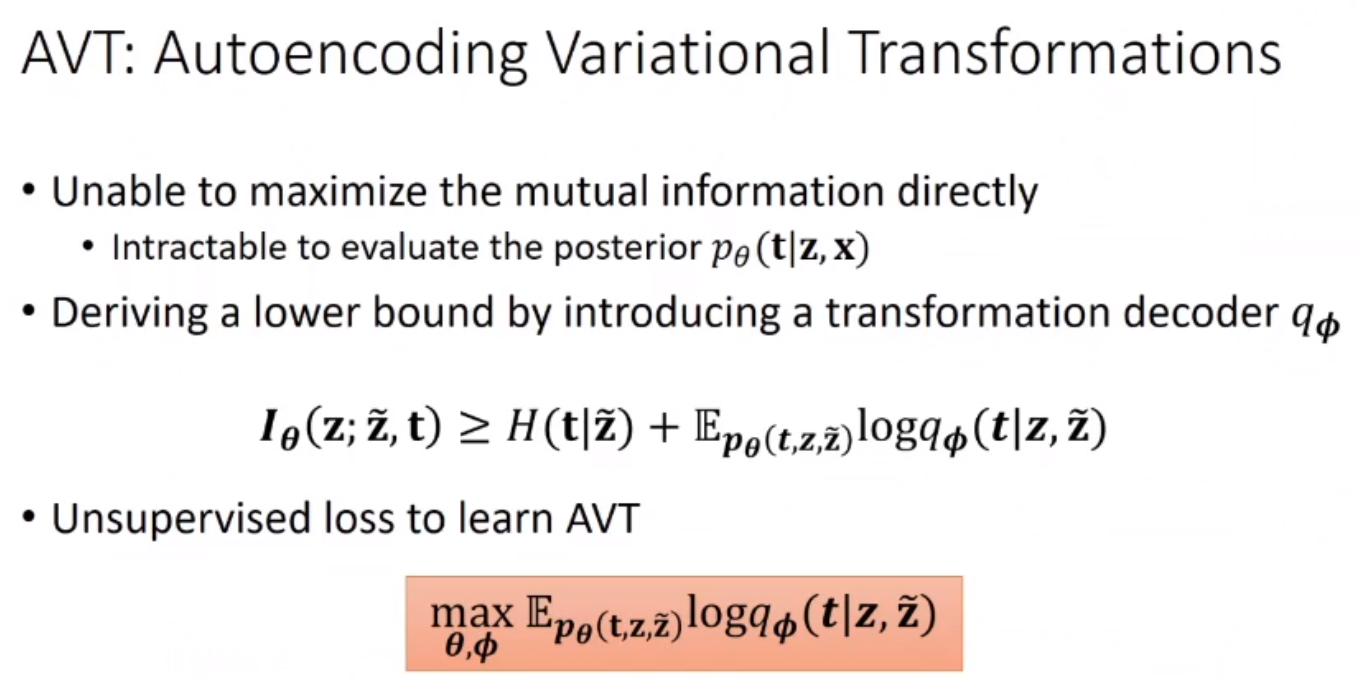
\includegraphics[width=0.8\paperwidth]{avt2.PNG}}
    \centerline{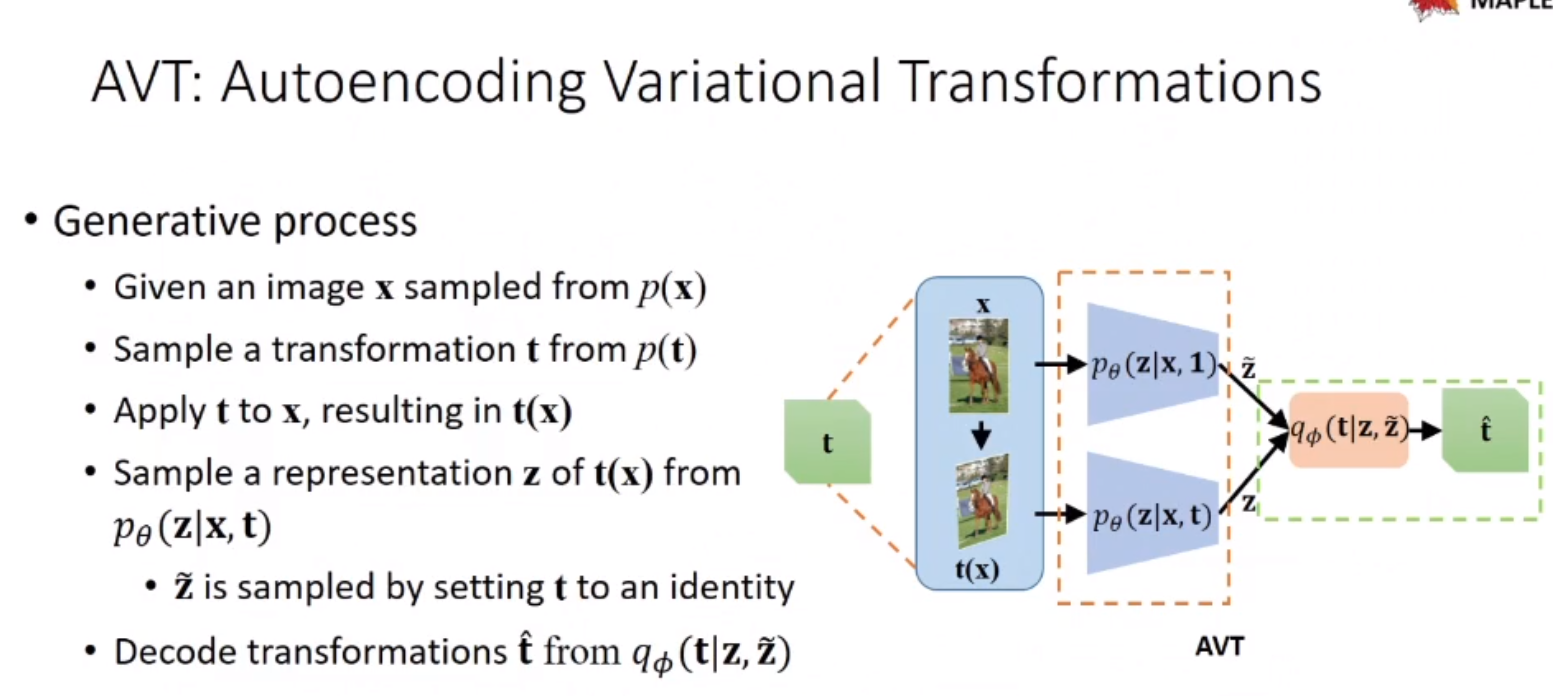
\includegraphics[width=0.8\paperwidth]{avt-training.PNG}}
    AVT:
    \begin{itemize}
        \item minimize $z, x$ mutual info \trarr maxmize $I_\theta(z; \tilde z, t)$
    \end{itemize}

    \centerline{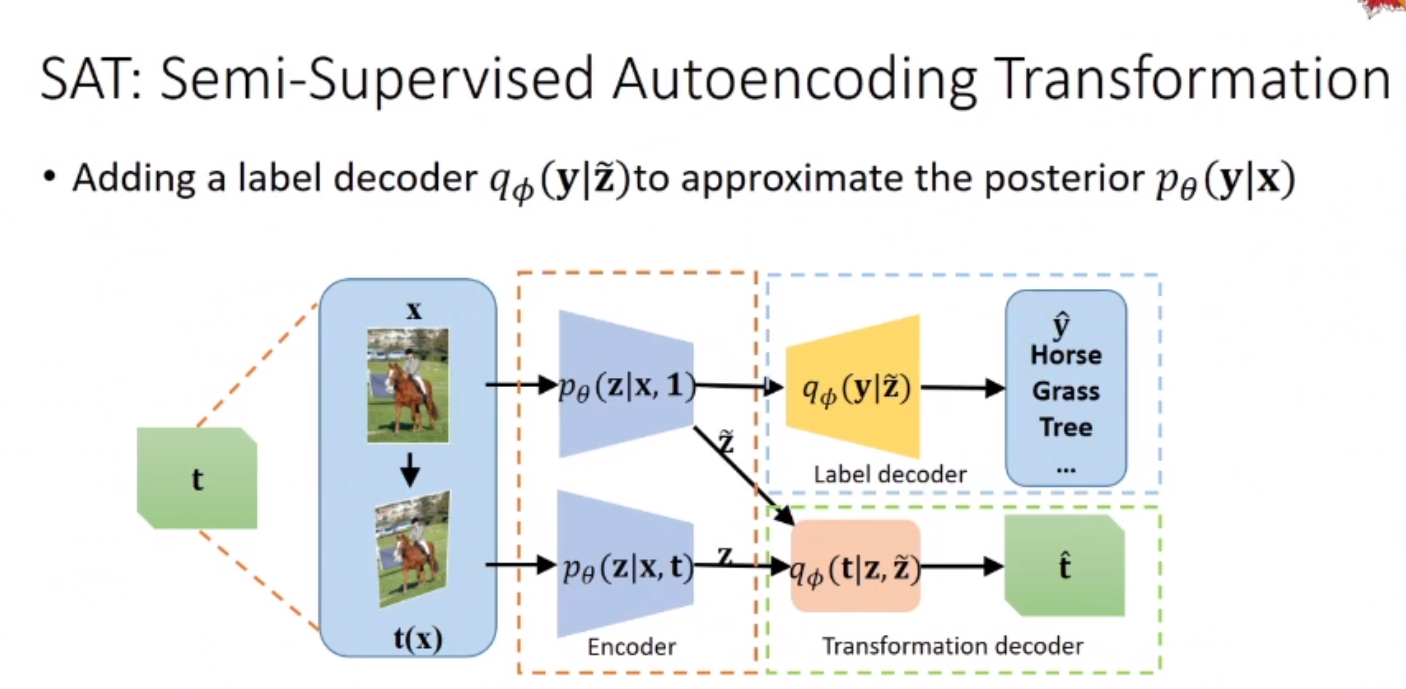
\includegraphics[width=0.8\paperwidth]{sat.PNG}}
    \centerline{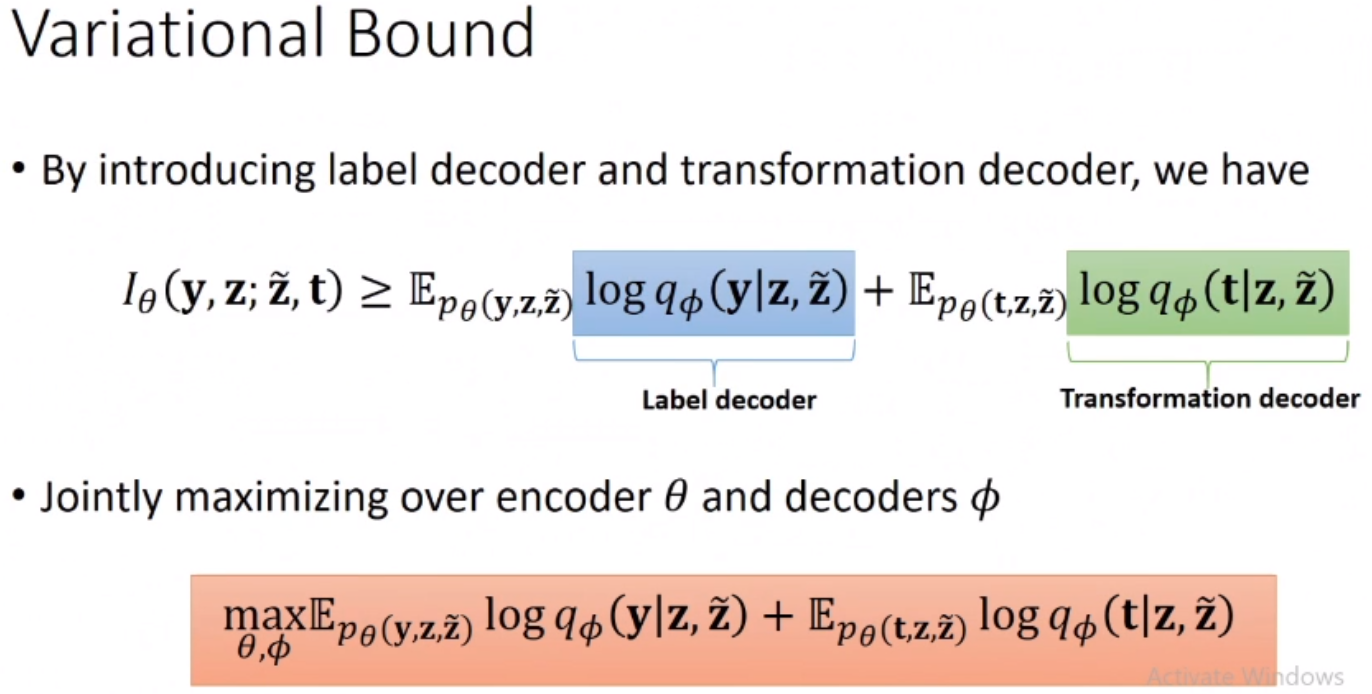
\includegraphics[width=0.8\paperwidth]{sat-loss.PNG}}
    SAT:
    \begin{itemize}
        \item add a label decoder compared to AVT.
        \item variational surrogate \trarr cross-entropy loss on supervised data + AVT loss
    \end{itemize}

    Contrastive Learning: more utilized trans-invariant repr.
    Future: unifying trans-inv/equiv repr.

\section{AET, AVT: Autoencoding Transformations}
    \bt{Idea} autoencoders used in modeling transformations rather than images in order to learn general repr.

    \centerline{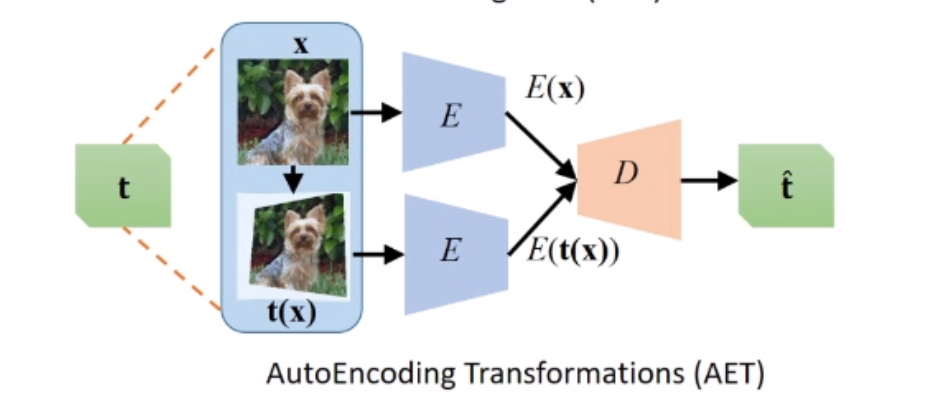
\includegraphics[width=0.8\paperwidth]{aet.PNG}}
    AET:\begin{itemize}
        \item use autoencoders to learn \bt{transformations}
        \item trans. generated randomly for self-supervised learing
        \item use Siamese net as encoder backbone
        \item AET loss: parameterized, non-parametric, GAN-induced
    \end{itemize}
    Losses in AET:
    \begin{itemize}
        \item parameterized transformations: if trans. are parameterized $\mathcal T \in \{t_\theta | \theta \in \Theta\}$, loss can be defined as norm of param. diff. $l(t_\theta, t_{\hat \theta}=||\theta - \hat \theta||_{\cdot})$
        \item for non-parametric trans., use expected distance on source domain $l(t, \hat t)=\mathbb E_{x\sim X}\{dist(t(x), \hat t(x)))\}$
        \item GAN-induced trans.: image tranformed in form $G(x, z)$, we have loss $l(t_z, t_{\hat z}=||z-\hat z||_\cdot)$
    \end{itemize}

    \bt{Idea of AVT} use prob. dist. to model trans., VAE like modeling!
    
    \centerline{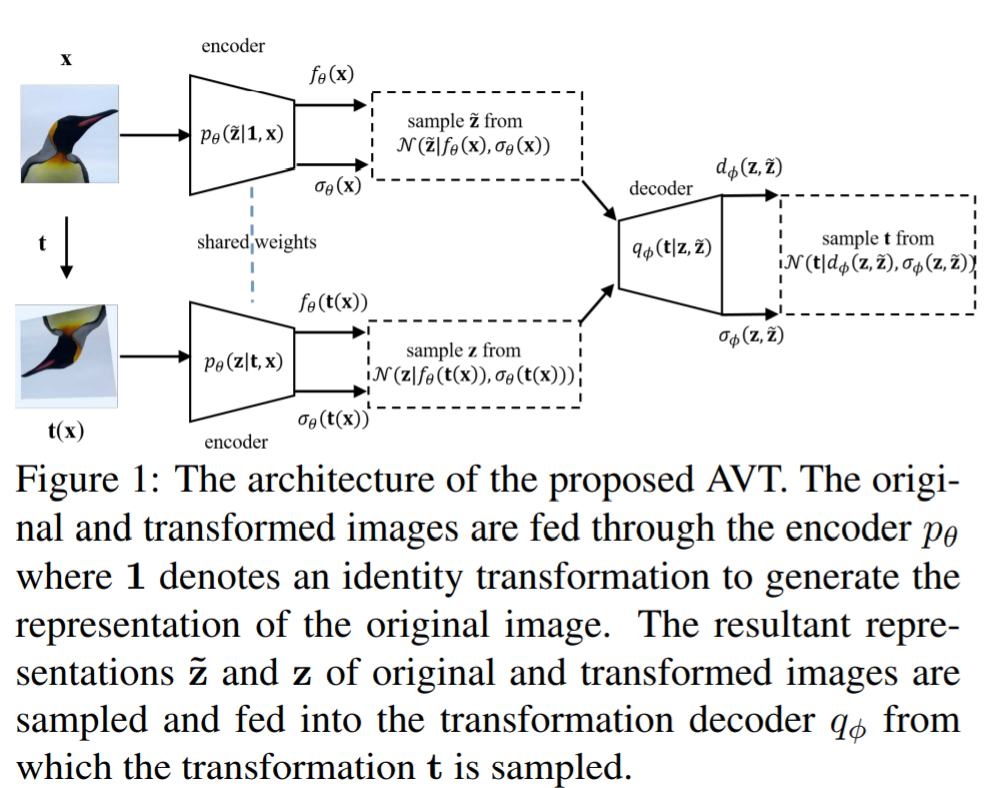
\includegraphics[width=0.8\paperwidth]{avt-arch.PNG}}
    AVT: \begin{itemize}
        \item maximize mutual info $I(t;z|\tilde z)$
        \item variational bound:
            \begin{align}
                I(t;z|\tilde z) &= H(t|\tilde z) - H(t|z, \tilde z)\\
                &= H(t|\tilde z) + \mathbb E_{p_\theta(t, z, \tilde z)}[p_\theta(t|z,\tilde z)]

            \end{align}
    \end{itemize}

\end{document}